%% Infografia_DCBI_2026_dark.tex — versión dark mode (pantalla / proyección)
%% Compilar desde Infografia/: pdflatex -interaction=nonstopmode Infografia_DCBI_2026_dark.tex

\documentclass[9pt,a4paper]{article}
\usepackage[margin=0.55cm,top=0.50cm,bottom=0.50cm]{geometry}
\usepackage[utf8]{inputenc}
\usepackage[T1]{fontenc}
\usepackage[spanish,mexico]{babel}
\decimalpoint
\usepackage{lmodern}
\renewcommand{\familydefault}{\sfdefault}
\usepackage{microtype}
\usepackage{amsmath,amssymb}
\usepackage{graphicx}
\graphicspath{{../}}
\usepackage{xcolor}
\usepackage{multicol}
\usepackage{tcolorbox}
\tcbuselibrary{skins}

\pagestyle{empty}
\parindent=0pt
\parskip=0pt
\setlength{\columnsep}{5pt}
\setlength{\multicolsep}{2pt}

%%─── Paleta nowhere_minimal — modo oscuro ────────────────────────────────────
\definecolor{uamred}{HTML}{C0101A}
\definecolor{nearblack}{HTML}{0D0D0D}
\definecolor{darkbg}{HTML}{141414}      %% fondo de página
\definecolor{graymid}{HTML}{8A8A8A}     %% texto secundario — más claro que en modo luz
\definecolor{paperbg}{HTML}{F5F4F0}     %% texto principal sobre fondo oscuro

%%─── Fondo oscuro de página ──────────────────────────────────────────────────
\pagecolor{darkbg}
\color{paperbg}

%%─── Escala tipográfica — texto claro sobre fondo oscuro ─────────────────────
\newcommand{\BIGNUM}[1]%
  {{\fontsize{20}{22}\selectfont\ttfamily\bfseries\color{uamred}#1}}
\newcommand{\BIGNUMK}[1]%
  {{\fontsize{20}{22}\selectfont\ttfamily\bfseries\color{paperbg}#1}}
\newcommand{\MEDNUM}[1]%
  {{\fontsize{14}{16}\selectfont\ttfamily\bfseries\color{uamred}#1}}
\newcommand{\MEDNUMK}[1]%
  {{\fontsize{14}{16}\selectfont\ttfamily\bfseries\color{paperbg}#1}}
\newcommand{\LBL}[1]{{\small\bfseries\color{paperbg}#1}}
\newcommand{\NOTE}[1]{{\tiny\color{graymid}#1}}
\newcommand{\SECHEAD}[1]{%
  {\fontsize{6}{7}\selectfont\bfseries\color{paperbg}\MakeUppercase{#1}}%
  \par\nointerlineskip\vspace{1pt}%
  {\color{uamred}\hrule height 0.6pt}\par\vspace{3pt}}

%%─── Estilos tcolorbox — modo oscuro ─────────────────────────────────────────
\tcbset{
  %% encabezado — rojo sólido, mismo que modo luz
  hdr/.style={enhanced,sharp corners,
    colback=uamred,colframe=uamred,
    colupper=white,
    left=7pt,right=7pt,top=5pt,bottom=5pt,
    before skip=0pt,after skip=3pt},
  %% tarjeta estadística — gris oscuro, borde norte rojo
  stat/.style={enhanced,sharp corners,
    colback=white!10!nearblack,colframe=white!10!nearblack,
    colupper=paperbg,
    borderline north={1.8pt}{0pt}{uamred},
    left=5pt,right=5pt,top=4pt,bottom=3pt,
    before skip=0pt,after skip=0pt},
  %% banda de sección — gris oscuro ligeramente más claro
  band/.style={enhanced,sharp corners,
    colback=white!14!nearblack,colframe=white!14!nearblack,
    colupper=paperbg,
    left=5pt,right=5pt,top=4pt,bottom=4pt,
    before skip=2pt,after skip=2pt},
  %% tarjeta de hallazgo — borde izquierdo rojo, fondo muy oscuro
  card/.style={enhanced,sharp corners,
    colback=white!7!nearblack,colframe=white!7!nearblack,
    colupper=paperbg,
    borderline west={2pt}{0pt}{uamred},
    left=5pt,right=4pt,top=3pt,bottom=3pt,
    before skip=2pt,after skip=0pt},
  %% contenedor de figura — borde gris medio, fondo casi negro
  figbox/.style={enhanced,sharp corners,
    colback=white!4!nearblack,colframe=white!28!nearblack,
    colupper=paperbg,
    left=2pt,right=2pt,top=2pt,bottom=2pt,
    before skip=0pt,after skip=0pt},
  %% caja sin decoración (mejora relativa, pie)
  plain/.style={enhanced,sharp corners,
    colback=white!10!nearblack,colframe=white!10!nearblack,
    colupper=paperbg,
    left=5pt,right=5pt,top=3pt,bottom=3pt,
    before skip=0pt,after skip=0pt},
  %% caja de lectura — borde norte gris, sin acento de color
  leer/.style={enhanced,sharp corners,
    colback=white!6!nearblack,colframe=white!6!nearblack,
    colupper=paperbg,
    borderline north={0.5pt}{0pt}{graymid},
    left=5pt,right=4pt,top=3pt,bottom=3pt,
    before skip=2pt,after skip=0pt},
}

\begin{document}

%%═══════════════════════════════════════════════════════════════════════════════
%% PÁGINA 1 — Corpus, proceso y resultados
%%═══════════════════════════════════════════════════════════════════════════════

%% ── Encabezado ───────────────────────────────────────────────────────────────
\begin{tcolorbox}[hdr]
{\fontsize{11.5}{13.5}\selectfont\bfseries\color{white}%
 ¿QUÉ TAN PARECIDOS SON LOS PROGRAMAS DE UEA ENTRE LAS LICENCIATURAS?}\\[1pt]
{\small\color{white!60!uamred}%
 Análisis de similitud de contenidos · Modificación curricular 2026 ·
 División de Ciencias Básicas e Ingeniería · UAM-Azcapotzalco}
\end{tcolorbox}

%% ── Tres estadísticas — multicols{3} en minipage ─────────────────────────────
\begin{minipage}[t]{\linewidth}
\begin{multicols}{3}
\begin{tcolorbox}[stat]
\centering
\BIGNUM{626}\\[1pt]
\LBL{programas de UEA analizados}\\[1pt]
\NOTE{773 inventariados · se excluyeron las UEAs del Tronco General}
\end{tcolorbox}
\columnbreak
\begin{tcolorbox}[stat]
\centering
\BIGNUMK{195\,375}\\[1pt]
\LBL{pares de programas comparados}\\[1pt]
\NOTE{Todas las combinaciones posibles de dos programas del corpus}
\end{tcolorbox}
\columnbreak
\begin{tcolorbox}[stat]
\centering
\BIGNUMK{1\,505}\\[1pt]
\LBL{pares revisados en detalle}\\[1pt]
\NOTE{Los pares más parecidos, verificados con análisis inteligente de contenido}
\end{tcolorbox}
\end{multicols}
\end{minipage}

\vspace{3pt}

%% ── Proceso de análisis ──────────────────────────────────────────────────────
\begin{tcolorbox}[band]
\SECHEAD{proceso de análisis en dos fases}
\centering\small\color{paperbg}
\textbf{Texto de 626 programas}~%
$\longrightarrow$~%
\textbf{Comparación por palabras clave}~%
$\longrightarrow$~%
\textbf{1\,505 pares candidatos}~%
$\longrightarrow$~%
\textbf{Revisión inteligente de contenido}~%
$\longrightarrow$~%
\textbf{Similitud real entre programas}
\end{tcolorbox}

\vspace{3pt}

%% ── Mapa de similitud entre planes + resultados ──────────────────────────────
\begin{minipage}[t]{\linewidth}
\begin{multicols}{2}
%% columna 1 — figura
\begin{tcolorbox}[figbox]
{\footnotesize\bfseries Nivel de similitud entre los 10 planes de estudio}%
\par\vspace{2pt}
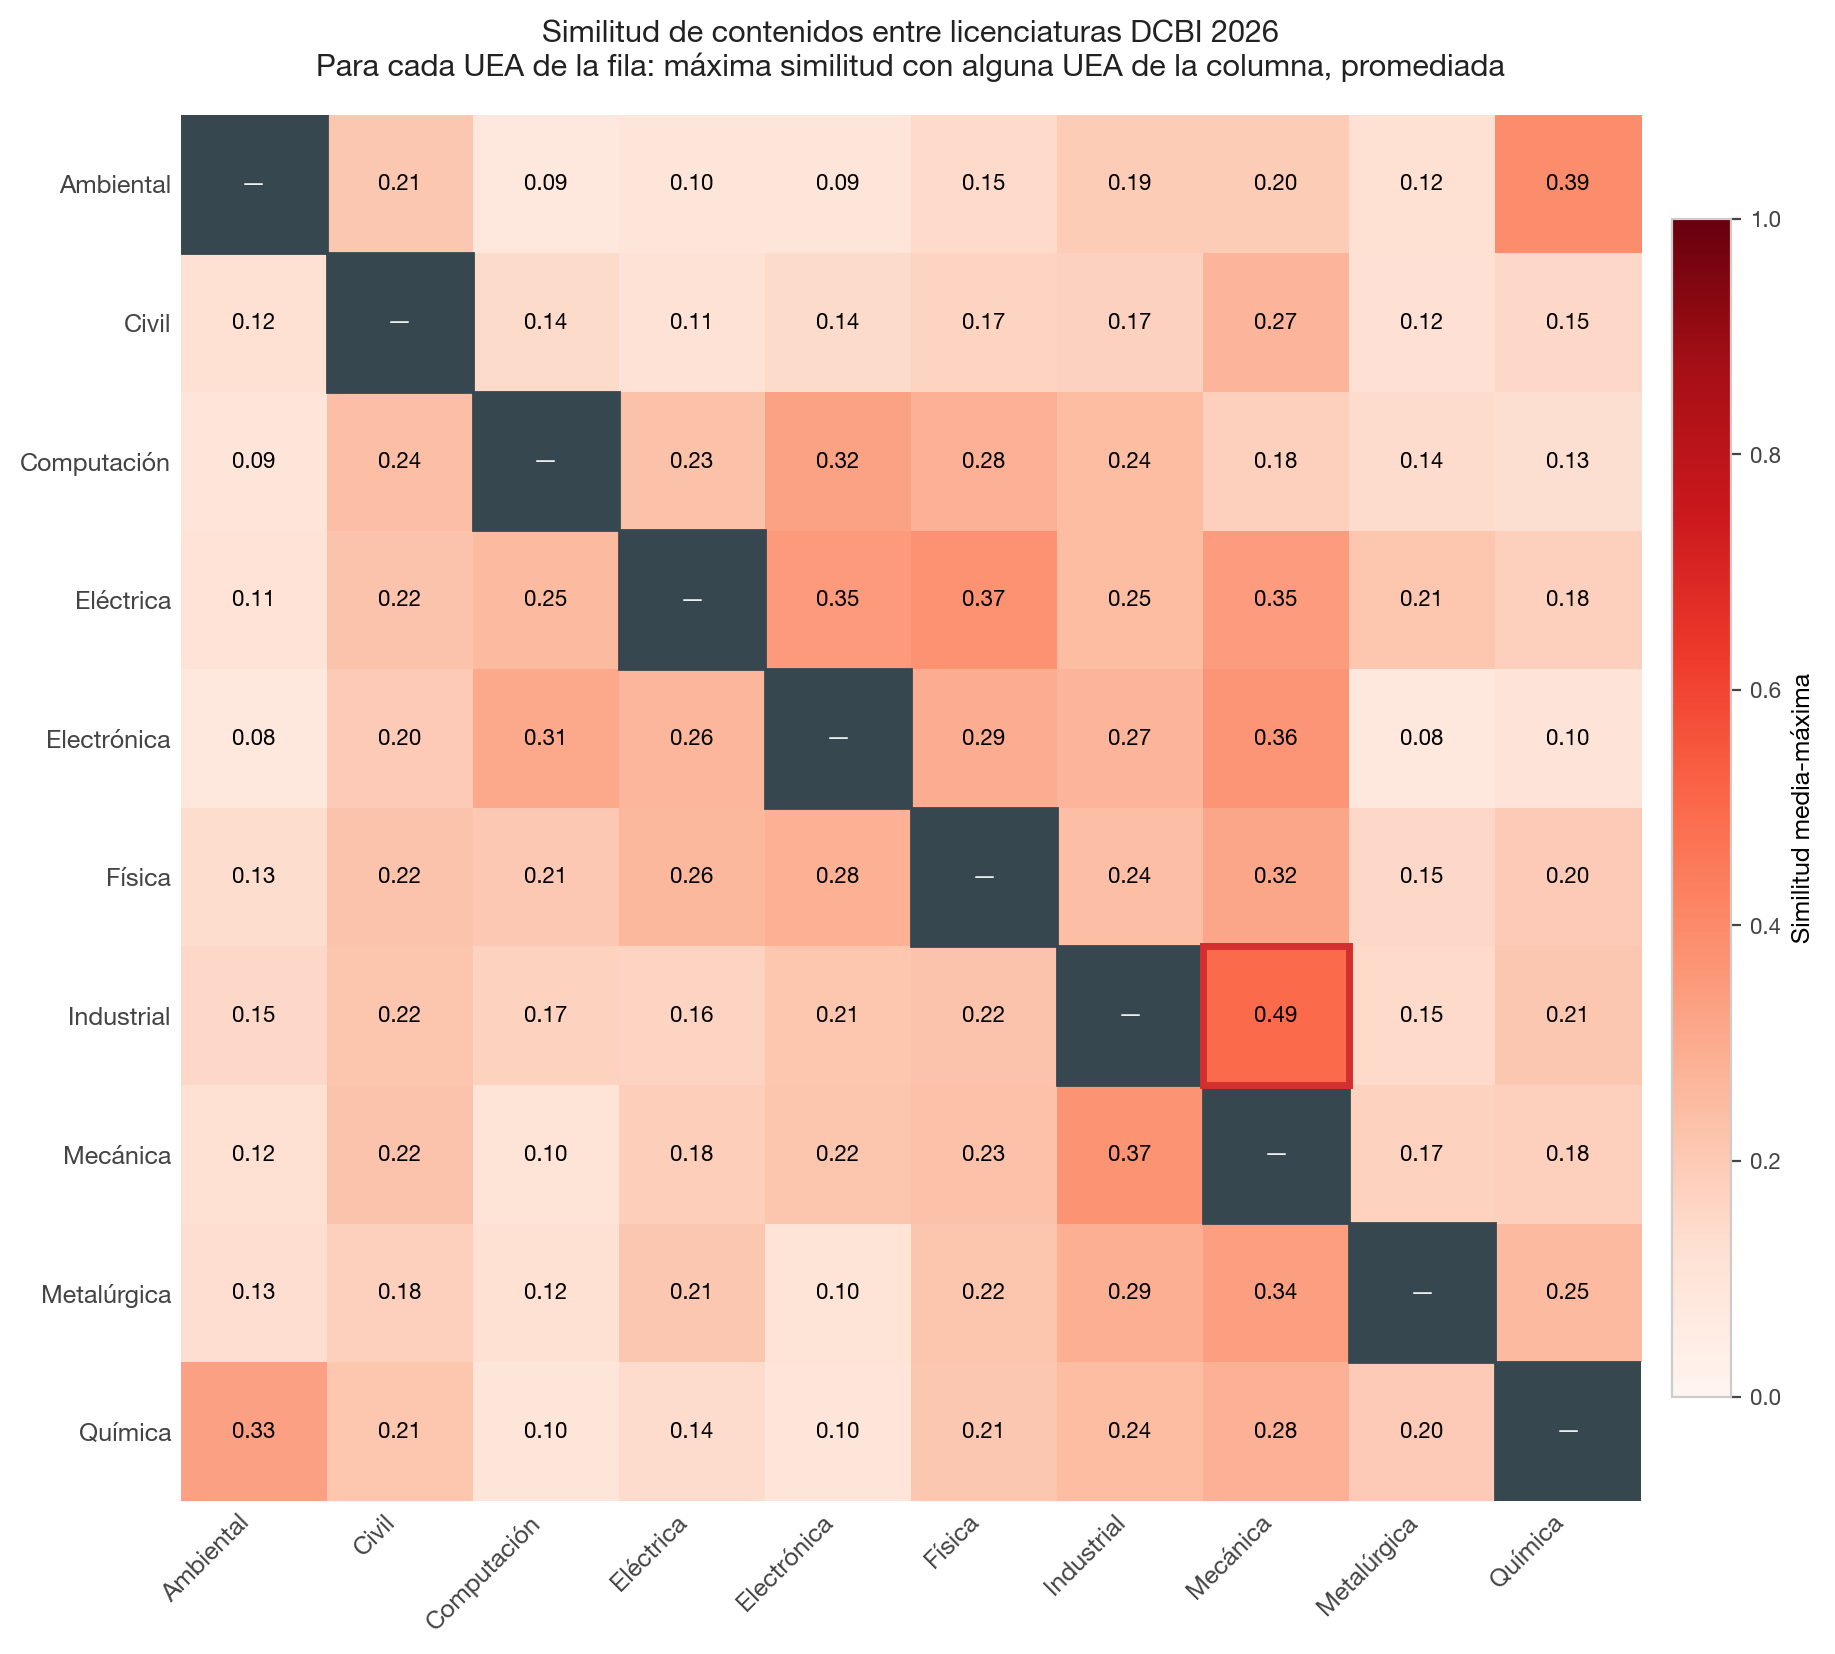
\includegraphics[width=\linewidth]{Figuras/heatmap_licenciaturas.png}
\par\vspace{1pt}
\NOTE{Amarillo\,=\,poca similitud;\;rojo intenso\,=\,contenidos muy parecidos o idénticos.
La diagonal siempre es roja: cada plan comparado consigo mismo.}
\end{tcolorbox}
\columnbreak
%% columna 2 — resultados
\SECHEAD{resultados del análisis}
\begin{tcolorbox}[card]
\MEDNUM{391}\;\LBL{pares similares entre licenciaturas}\\
\NOTE{programas de UEA con contenido muy parecido entre planes distintos}
\end{tcolorbox}
\begin{tcolorbox}[card]
\MEDNUMK{217}\;\LBL{pares similares dentro de un plan}\\
\NOTE{programas de UEA muy parecidos dentro de la misma licenciatura}
\end{tcolorbox}
\begin{tcolorbox}[card]
\MEDNUMK{455}\;\LBL{pares encontrados solo por contenido}\\
\NOTE{la comparación por palabras clave no los hubiera detectado}
\end{tcolorbox}
\vspace{3pt}
\begin{tcolorbox}[plain]
\centering
\MEDNUMK{+154\,\%}\;\small\color{paperbg} más pares entre licenciaturas\\[-1pt]
\NOTE{vs.\ solo comparar palabras clave}\\[3pt]
\MEDNUMK{+75\,\%}\;\small\color{paperbg} más pares dentro de cada plan\\[-1pt]
\NOTE{vs.\ solo comparar palabras clave}
\end{tcolorbox}
\begin{tcolorbox}[leer]
{\tiny\bfseries Cómo leer}\par\vspace{1pt}
\NOTE{Busca las celdas más oscuras \emph{fuera} de la diagonal — ahí están los pares de licenciaturas que más contenido comparten.
La diagonal siempre es rojo intenso: es cada licenciatura comparada consigo misma.}
\end{tcolorbox}
\end{multicols}
\end{minipage}

\vspace{3pt}

%% ── Mapa de conteo + casos extremos ─────────────────────────────────────────
\begin{minipage}[t]{\linewidth}
\begin{multicols}{2}
%% columna 1 — figura
\begin{tcolorbox}[figbox]
{\footnotesize\bfseries Número de programas casi idénticos entre cada par de licenciaturas}%
\par\vspace{2pt}
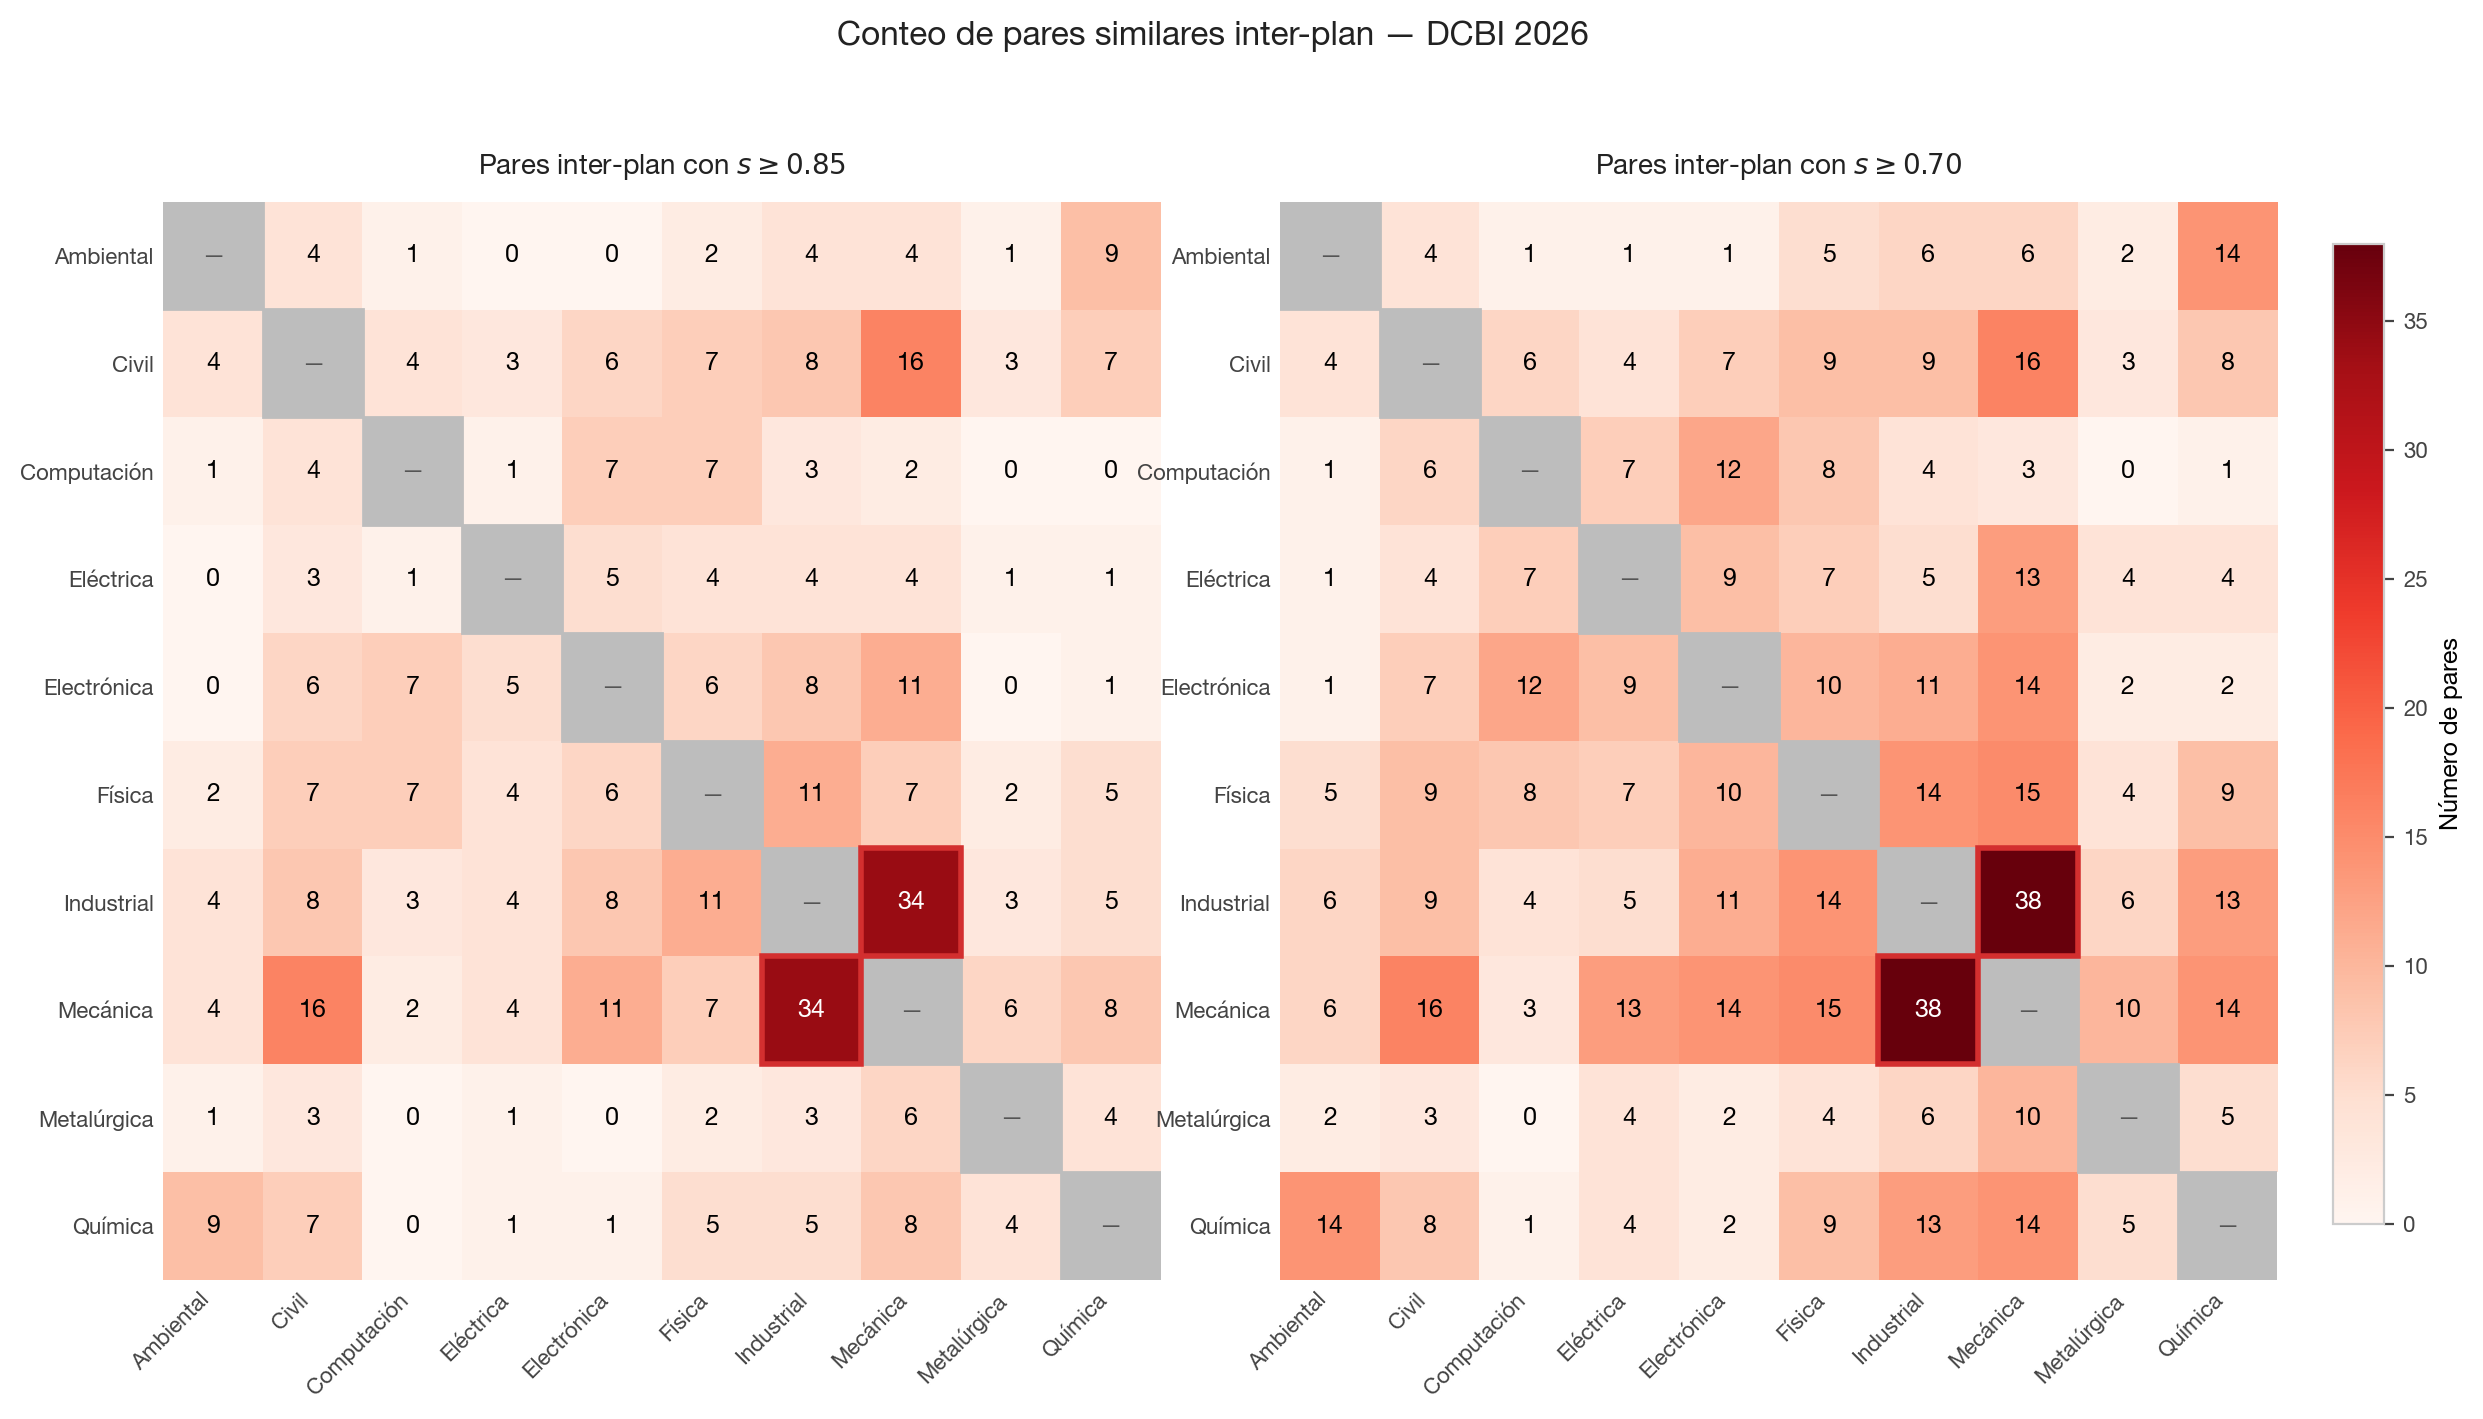
\includegraphics[width=\linewidth]{Figuras/heatmap_interplan_conteo.png}
\par\vspace{1pt}
\NOTE{Panel izquierdo: criterio estricto (casi idénticos).
Panel derecho: criterio más amplio (muy similares).
Industrial–Mecánica: \textbf{38 programas} compartidos.}
\end{tcolorbox}
\columnbreak
%% columna 2 — extremos
\SECHEAD{los casos más llamativos}
\begin{tcolorbox}[card]
{\footnotesize\bfseries El par con más programas en común}\\[1pt]
{\small Industrial\,--\,Mecánica}\\
\MEDNUM{38}\;\NOTE{programas muy similares}\quad
\MEDNUMK{34}\;\NOTE{casi idénticos}
\end{tcolorbox}
\begin{tcolorbox}[card]
{\footnotesize\bfseries Otros pares destacados}\\[1pt]
{\small Civil\,--\,Mecánica:\;\textbf{16}\,\NOTE{programas en común}}\\
{\small Ambiental\,--\,Química:\;\textbf{14}\,\NOTE{programas en común}}
\end{tcolorbox}
\begin{tcolorbox}[card]
{\footnotesize\bfseries El par sin ningún programa en común}\\[1pt]
{\small Computación\,--\,Metalúrgica}\\
\MEDNUMK{0}\;\NOTE{programas similares detectados}
\end{tcolorbox}
\end{multicols}
\end{minipage}
\vspace{3pt}
\begin{tcolorbox}[leer]
{\footnotesize\bfseries Cómo leer este mapa}\par\vspace{2pt}
{\footnotesize Cada celda muestra cuántos programas son casi idénticos entre ese par de licenciaturas.
El \textbf{panel izquierdo} aplica el criterio más estricto (casi idénticos);
el \textbf{panel derecho}, el criterio más amplio (muy similares).
Cuanto más oscura la celda, más programas comparten esas dos licenciaturas.
Una celda en blanco significa que no se encontró contenido compartido.}
\end{tcolorbox}

\newpage

%%═══════════════════════════════════════════════════════════════════════════════
%% PÁGINA 2 — Hallazgos principales
%%═══════════════════════════════════════════════════════════════════════════════

%% ── Encabezado ───────────────────────────────────────────────────────────────
\begin{tcolorbox}[hdr]
{\fontsize{11.5}{13.5}\selectfont\bfseries\color{white}HALLAZGOS PRINCIPALES}\\[1pt]
{\small\color{white!60!uamred}%
Análisis de similitud de contenidos · División de Ciencias Básicas e Ingeniería · 626 programas de UEA}
\end{tcolorbox}

\vfill

%% ── Red de similitud + hallazgos entre licenciaturas ────────────────────────
\SECHEAD{similitudes entre licenciaturas distintas}
\begin{minipage}[t]{\linewidth}
\begin{multicols}{2}
%% columna 1 — grafo
\begin{tcolorbox}[figbox]
{\footnotesize\bfseries Red de licenciaturas con programas en común
(al menos 5 programas muy similares)}\par\vspace{2pt}
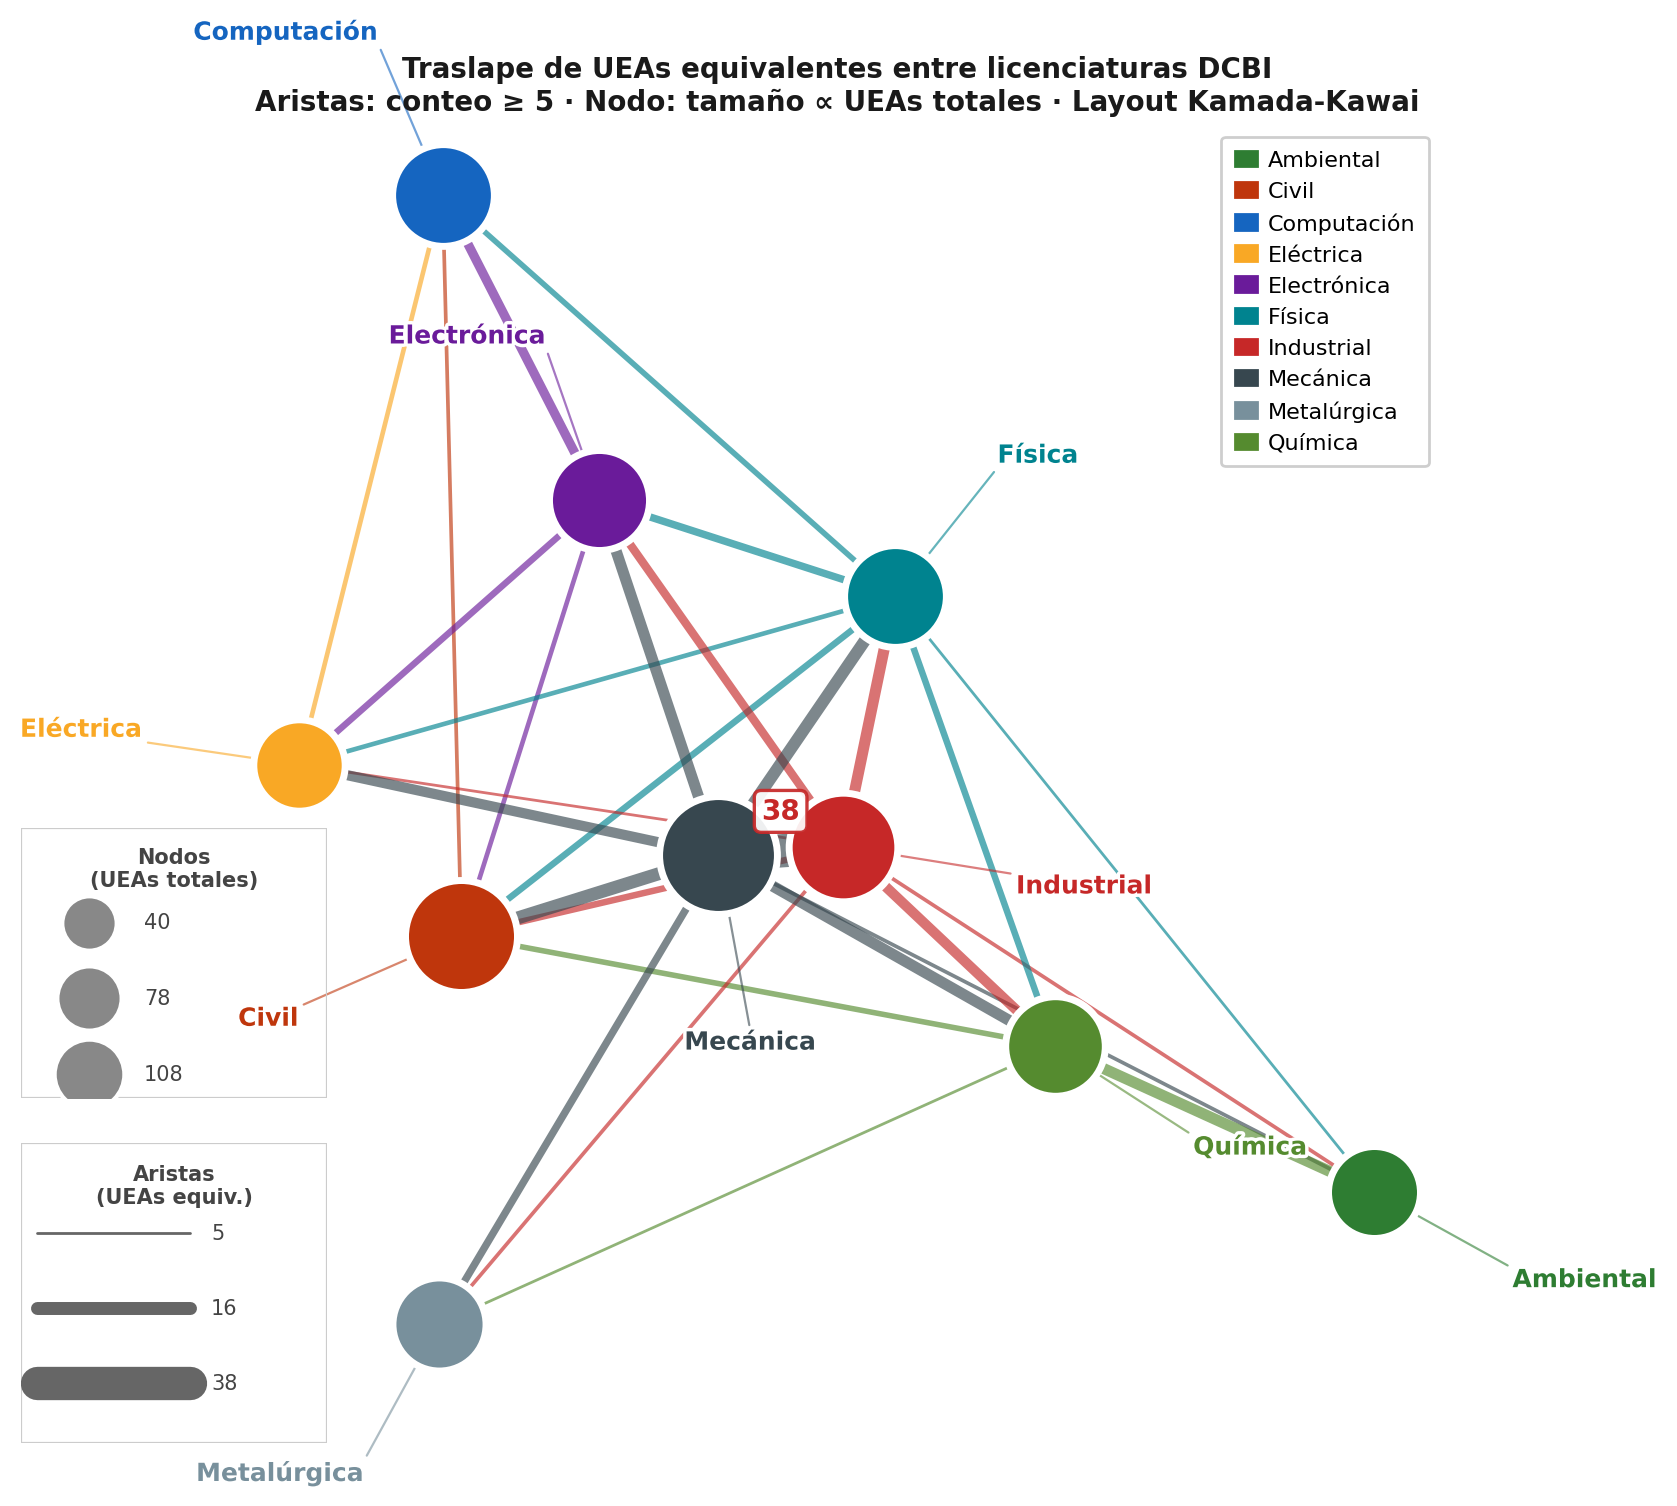
\includegraphics[width=\linewidth]{Figuras/grafo_licenciaturas_variante_B.png}
\par\vspace{1pt}
\NOTE{29 de los 45 pares posibles comparten 5 o más programas equivalentes.
Las líneas más gruesas unen los pares con mayor traslape de contenidos.}
\end{tcolorbox}
\columnbreak
%% columna 2 — H1–H4
\begin{tcolorbox}[card]
{\footnotesize\bfseries H1\;·\;Industrial\,--\,Mecánica}\\[2pt]
\BIGNUM{38}\;\LBL{programas muy similares}\\
\NOTE{34 prácticamente idénticos · manufactura, materiales,
termodinámica, cálculo numérico}
\end{tcolorbox}
\begin{tcolorbox}[card]
{\footnotesize\bfseries H2\;·\;Física — el plan más conectado}\\[2pt]
\BIGNUM{100}\;\LBL{pares con otras licenciaturas}\\
\NOTE{Comparte contenidos con los diez planes de la División.
Es el nodo con mayor conectividad.}
\end{tcolorbox}
\begin{tcolorbox}[card]
{\footnotesize\bfseries H3\;·\;Grupo de ingenierías clásicas}\\[2pt]
\NOTE{Mecánica, Industrial, Física y Electrónica comparten
10 o más programas entre sí.
Civil\,--\,Mecánica: 16 programas en común.}
\end{tcolorbox}
\begin{tcolorbox}[card]
{\footnotesize\bfseries H4\;·\;Ambiental\,--\,Química}\\[2pt]
\MEDNUMK{14}\;\LBL{programas muy similares}\\
\NOTE{9 prácticamente idénticos · ambos planes comparten
un núcleo implícito de ingeniería ambiental.}
\end{tcolorbox}
\end{multicols}
\end{minipage}
\vspace{3pt}
\begin{tcolorbox}[leer]
{\footnotesize\bfseries Cómo leer la red}\par\vspace{2pt}
{\footnotesize Cada punto en la red es una licenciatura.
Una línea aparece cuando dos planes comparten al menos 5 programas equivalentes;
cuanto más \textbf{gruesa la línea}, más programas tienen en común.
Las licenciaturas con más conexiones comparten contenidos con más planes de la División.
Física es la más conectada: tiene vínculos con los diez planes.}
\end{tcolorbox}

\vfill

%% ── H5–H8 Materias que se repiten en varios planes ───────────────────────────
\begin{tcolorbox}[band]
\SECHEAD{materias que se repiten en varios planes — sin coordinación entre licenciaturas}
\begin{minipage}[t]{\linewidth}
\begin{multicols}{2}
\raggedcolumns
{\footnotesize\bfseries Ecuaciones Diferenciales}\par\vspace{2pt}
\BIGNUMK{9\,/\,10}{\tiny\;planes}\par\vspace{2pt}
\NOTE{Contenido prácticamente idéntico en 9 licenciaturas.
Cada una la registra con su propia clave, sin coordinación formal entre los planes.}
\par\vspace{5pt}
{\footnotesize\bfseries Liderazgo y Emprendimiento}\par\vspace{2pt}
\BIGNUMK{9\,/\,10}{\tiny\;planes}\par\vspace{2pt}
\NOTE{Contenido muy similar en 9 licenciaturas.
Solo detectable mediante revisión del significado:
la comparación por palabras clave no lo detecta.}
\columnbreak

{\footnotesize\bfseries Educación Ambiental y Cambio Climático}\par\vspace{2pt}
\BIGNUMK{${\geq}$6}{\tiny\;planes}\par\vspace{2pt}
\NOTE{Contenido casi idéntico en seis licenciaturas:
Civil, Eléctrica, Electrónica, Física, Mecánica, Química.}
\par\vspace{5pt}
{\footnotesize\bfseries Núcleo matemático (3 materias)}\par\vspace{2pt}
\BIGNUMK{5}{\tiny\;planes c/u}\par\vspace{2pt}
\NOTE{Tres materias son prácticamente idénticas en cinco planes:
Probabilidad y Estadística ·
Métodos Numéricos · Programación Aplicada a Ingeniería.}
\end{multicols}
\end{minipage}
\end{tcolorbox}

\vfill

%% ── H10–H14 Similitudes dentro del mismo plan ────────────────────────────────
\begin{tcolorbox}[band]
\SECHEAD{programas duplicados o muy similares dentro del mismo plan de estudios}
\begin{minipage}[t]{\linewidth}
\begin{multicols}{2}
\raggedcolumns
{\footnotesize\bfseries 3 duplicados exactos encontrados}\par\vspace{2pt}
\NOTE{%
  \textbf{Química:} Análisis de Ciclo de Vida — el programa es idéntico en dos UEAs\\[1pt]
  \textbf{Física:} Aplicaciones Experimentales I y II — contenido idéntico\\[1pt]
  \textbf{Industrial:} una misma clave registrada dos veces}
\par\vspace{5pt}
{\footnotesize\bfseries Civil: 61 pares similares}\par\vspace{2pt}
\NOTE{El mayor número de programas parecidos dentro de un mismo plan.
La comparación por palabras detectaba solo 8;
la revisión de contenido encontró 61.
Estructuras, hidráulica y geotecnia.}
\columnbreak

{\footnotesize\bfseries Computación: 24 alertas descartadas}\par\vspace{2pt}
\NOTE{La comparación por palabras encontró 57 pares parecidos;
la revisión de contenido confirmó 33 y descartó 24.
El vocabulario genérico de programación
generaba similitudes aparentes que no eran reales.}
\par\vspace{5pt}
{\footnotesize\bfseries Metalúrgica: de 3 a 29 pares}\par\vspace{2pt}
\NOTE{El mayor salto relativo de todo el análisis.
El vocabulario técnico varía entre versiones de la misma materia,
pero el contenido es el mismo.
La revisión de significado revela los pares taller/teoría
que la comparación por palabras no detectaba.}
\end{multicols}
\end{minipage}
\end{tcolorbox}

\vfill

%% ── Pie ──────────────────────────────────────────────────────────────────────
\begin{tcolorbox}[plain]
\centering
{\footnotesize\color{graymid}Figuras interactivas y datos completos:}\quad
{\footnotesize\bfseries\color{uamred}\ttfamily cslmuam.github.io/similitud-dcbi-2026}
\end{tcolorbox}

\end{document}
